\subsection{Discovering the Far Field: Antenna Adventures!}

\begin{tcolorbox}[colback=gray!10, colframe=black, title=E9B08] What is the far field of an antenna?
\begin{enumerate}[label=\Alph*.]
    \item The region of the ionosphere where radiated power is not refracted
    \item The region where radiated power dissipates over a specified time period
    \item The region where radiated field strengths are constant
    \item \textbf{The region where the shape of the radiation pattern no longer varies with distance}
\end{enumerate} \end{tcolorbox}

\subsubsection{Related Concepts}

To understand what the far field of an antenna is, we first need to consider the concepts of radiated power and radiation patterns in antenna theory. Antennas convert input power into electromagnetic waves, which propagate through space. The behavior of these waves varies considerably depending on the distance from the antenna, and this is where the concept of different regions of an antenna’s radiation comes into play.

\subsubsection*{Near Field and Far Field:}

1. \textbf{Near Field:}: The region very close to the antenna (typically within a distance of one wavelength) where the emitted electromagnetic fields are complex and vary with both distance and angle.
   
2. \textbf{Far Field:}: This is the region where the emitted electromagnetic wave can be considered planar and far away from any effects from the antenna structure itself. Here, the characteristics of the field (such as directionality) become stable.

\subsubsection*{Radiation Pattern:}

The radiation pattern of an antenna describes how the power radiates into the surrounding space. In the far field, the shape of this pattern is fixed, and typical measurements (like gain) can be safely made since the distance from the antenna minimizes variation. 

\subsubsection*{Importance of the Far Field:}

Understanding the far field is crucial for applications such as radio communications, as it affects the range and efficiency of antennas. Typically, the far field begins at a distance that is twice the largest dimension of the antenna, this can be approximated using the following formula:

\[
d = \frac{2D^2}{\lambda}
\]

where:
- \( d \) is the distance to the far field,
- \( D \) is the largest linear dimension of the antenna,
- \( \lambda \) is the wavelength of the radiated signal.

\subsubsection*{Calculation Example:}

If we have a dipole antenna that is 1 meter long and we want to find the starting point of the far field at a frequency of 300 MHz (where the wavelength can be calculated as follows):

1. Calculate the wavelength \( \lambda \):

\[
\lambda = \frac{c}{f}
\]

where \( c \) is the speed of light (\(3 \times 10^8\, \text{m/s}\)) and \( f \) is the frequency. 

\[
\lambda = \frac{3 \times 10^8\, \text{m/s}}{300 \times 10^6\, \text{Hz}} = 1\, \text{m}
\]

2. Now using the formula to find \( d \):

\[
d = \frac{2D^2}{\lambda} = \frac{2 \cdot (1\, \text{m})^2}{1\, \text{m}} = 2\, \text{m}
\]

Thus, the far field region starts at approximately 2 meters from the antenna.

\subsubsection{Conclusion}

In conclusion, knowing that the far field is the region where the shape of the radiation pattern no longer varies with distance is essential for understanding antenna operation and designing effective communication systems. This knowledge allows engineers to optimize signal coverage and quality in practical applications.

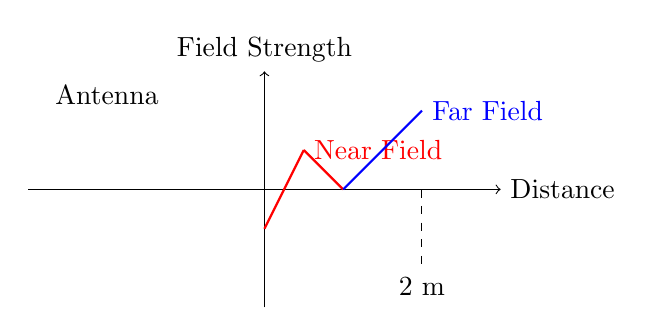
\begin{tikzpicture}
    \draw[->] (-3,0) -- (3,0) node[right] {Distance};
    \draw[->] (0,-1.5) -- (0,1.5) node[above] {Field Strength};
    
    % Draw near field region
    \draw[red, thick] (0,-0.5) -- (0.5,0.5) node[right] {Near Field};
    \draw[red, thick] (0.5,0.5) -- (1,0);
    
    % Draw far field region
    \draw[blue, thick] (1,0) -- (2,1) node[right] {Far Field};
    
    % Mark 2 meters
    \draw[dashed] (2,0) -- (2,-1) node[below] {2 m};
    
    % Label
    \node at (-2, 1.2) {Antenna};
\end{tikzpicture}
